\documentclass[11pt]{exam}

\usepackage{amsmath, amssymb, amsthm, multicol}
\usepackage{graphicx}
\usepackage{textcomp}
\usepackage{tikz}
\usepackage{mathrsfs}
%\usepackage[top=1in, bottom=1in, left=1in, right=1in]{geometry}
%\usepackage{framed}


%\newenvironment{ques}[2]{\vskip 1ex \noindent{\bf Question #1:}\marginpar{(#2 pts)}}{}
%\newenvironment{sol}{\begin{framed} \noindent{\em Solution:}}{\end{framed}\vskip 1em}



\def\d{\displaystyle}
\def\b{\mathbf}
\def\N{\mathbb{N}}
\def\R{\mathbb{R}}
\def\Z{\mathbb{Z}}
\def\Q{\mathbb{Q}}
\def\C{\mathbb{C}}
\def\F{\mathscr{F}}
\def\st{~:~}
\def\bar{\overline}
\def\inv{^{-1}}
\def\imp{\rightarrow}
\def\and{\wedge}
\def\onto{\twoheadrightarrow}
\DeclareMathOperator{\Gal}{Gal}


%\pointname{pts}
\pointsinmargin
\marginpointname{pts}
\marginbonuspointname{bns-pts}
\addpoints
\pagestyle{head}
%\printanswers

\firstpageheader{MATH 322}{\bf Homework 3}{Due: Wednesday, February 13}




\begin{document}

\noindent \textbf{Instructions}: Carefully write up solutions to the questions below.  A solution should consist of both the answer and a careful explanation for why that answer must be correct.  Any solutions without an explanation written out in English prose will receive no credit.  You are welcome to work together, but write up solutions in your own, individual rules.  Also, NO INTERNET!
\vskip 1ex
\begin{questions}






\question[4] Suppose $E$ is a degree 2 extension of $F$.  Prove that $E$ is the splitting field for some polynomial in $F[x]$.

\begin{solution}
If $E$ is a degree 2 extension of $F$, then $E = F(c)$ where $c$ is the root to some irreducible degree 2 polynomial, $p(x)$.  We claim that $E$ is actually the splitting field for $p(x)$.  Note that in $E$, we can factor $p(x)$ as $(x-c)q(x)$ where $q(x)$ is a degree 1 polynomial with coefficients in $E$.  But this means that $q(x)$ has a root in $E$ as well: if $q(x) = ax + b$ then $\frac{b}{a}$ is a root, which is in $E$ because $a$ and $b$ are.  Thus $E$ contains all the roots of $p(x)$, as required.
\end{solution}



\question[6] Let $p(x)$ be a polynomial of degree $n$ in $F[x]$ for some field $F$.  Prove that there is a splitting field $E$ for $p(x)$ such that $[E:F] \le n!$.  Your proof must use \textbf{mathematical induction}!  Let $P(n)$ be the statement, ``If $p(x)$ has degree $n$, then there is a splitting field with degree no more than $n!$'' and prove $P(n)$ is true for all $n \ge 1$.  

\begin{solution}
We know that we can always find an extension of $F$ of degree at most $n$ (exactly $n$ if $p(x)$ is irreducible) which contains a root of $p(x)$.  In this larger field, we can factor $p(x)$ as $(x-c)q(x)$ where $c$ is the newly adjoined root of $p(x)$.  We now know that $q(x)$ has degree $n-1$.  Now repeat.  To make this rigorous, use induction.  

For the base case, it is clear that any polynomial of degree 1 has a splitting field $E$ with $[E:F] \le 1$, since $E = F$ works.  Now assume that the proposition is true for all polynomials of degree $k$.  Consider $p(x)$ of degree $k+1$.  Find an extension $F_1$ of $F$ in which $p(x)$ has a root.  Factor $p(x) = (x-c)q(x)$ in $F_1[x]$.  We have that $[F_1:F] \le k+1$.  Now $q(x)$ is a polynomial of degree $k$, so we can apply our induction hypothesis to conclude that there is a splitting field $E$ for $q(x)$ extending $F_1$ with $[E:F_1] \le k!$.  But $E$ contains all the roots of $q(x)$, as well as $c$ (the other root of $p(x)$) so $E$ is a splitting field for $p(x)$ extending $F$.  By the tower rule, $[E:F]\le (k+1)!$.
\end{solution}

%\question Let $\varphi:F\to F$ be an automorphism.  Prove that if $f(a) = b$, then $a$ and $b$ are roots to the same polynomial.  That is, any polynomial that has $a$ as a root also has $b$ are a root.
\question[8] Consider the field $\Q(\sqrt[4]{3}, i)$. 
\begin{parts}
	 \part Is this a splitting field for some polynomial in $\Q[x]$?  If so, what is the degree of that polynomial? 
	 \begin{solution}
		 Yes, since in this field $x^4 - 3$ factors completely (its roots are $\pm \sqrt[4]{3}$ and $\pm \sqrt[4]{3}i$).  So it is the splitting field of a degree 4 polynomial.  
		 
		 It is also the splitting field of a degree 8 polynomial.  We know there is some element $\alpha$ of the field such that $\Q(\alpha)$ is the field.  This number will have a degree 8 minimal polynomial, and that polynomial will split completely in the field.
	 \end{solution}
	 \part What is the degree $[\Q(\sqrt[4]{3}, i):\Q]$?  Explain how you know.
	 \begin{solution}
		 This is degree 8.  We know that $\Q(\sqrt[4]{3})$ has degree 4 over $\Q$, but that this is only real, so adding $i$ will be more than a degree 1 extension.  However, $i$ has minimal polynomial $x^2 + 1$, so it will be a degree 2 extension of $\Q(\sqrt[4]{3})$.  Using the tower rule, we get degree 8.
	 \end{solution}
	 \part Draw as much of a complete tower diagram as you can describing the fields between $\Q$ and $\Q(\sqrt[4]{3}, i)$.
	 \begin{solution}
		 You don't need to have all of this, but here is the complete tower diagram for this field.
		 \begin{center}
		 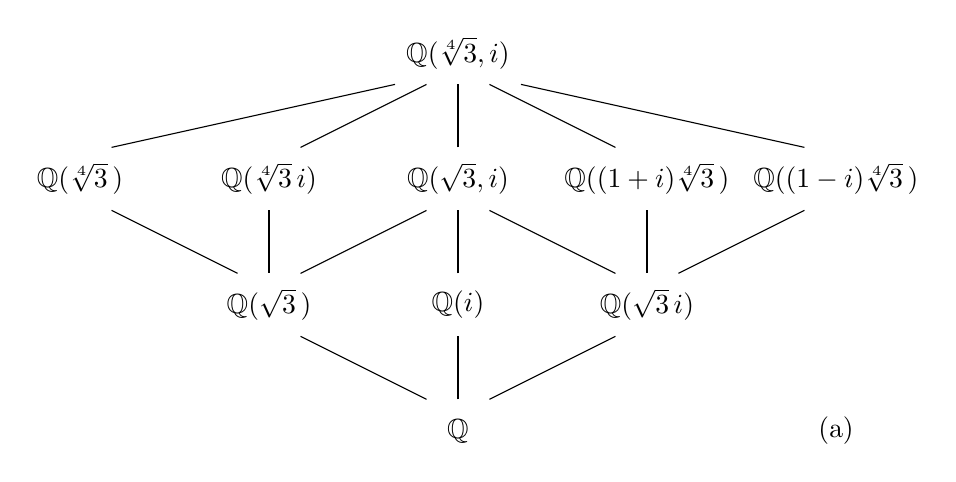
\begin{tikzpicture}[scale=0.8]

% \draw  (-1,0.5) -- (-5.5,1.5);
% \draw  (-0.5,0.5) -- (-2.5,1.5);
% \draw  (0,0.5) -- (0,1.5);
% \draw  (0.5,0.5) -- (2.5,1.5);
% \draw  (1,0.5) -- (5.5,1.5);
% 
% \draw  (-5.5,2.5) -- (-3.5,3.5);
% \draw  (-3,2.5) -- (-3,3.5);
% \draw  (-0.5,2.5) -- (-2.5,3.5);
% \draw  (0,2.5) -- (0,3.5);
% \draw  (5.5,2.5) -- (3.5,3.5);
% \draw  (3,2.5) -- (3,3.5);
% \draw  (0.5,2.5) -- (2.5,3.5);
% \draw  (3,2.5) -- (3,3.5);
% 
% \draw  (-3,4.5) -- (-0.5,5.5);
% \draw  (0,4.5) -- (0,5.5);
% \draw  (3,4.5) -- (0.5,5.5);
% 
% \node at (0,0)  {$\{  \identity \}$};
% \node at (-6,2)  {$\{  \identity, \tau \}$};
% \node at (-3,2)  {$\{  \identity, \sigma^2 \tau \}$};
% \node at (0,2)  {$\{  \identity, \sigma^2 \}$};
% \node at (3,2)  {$\{  \identity, \sigma \tau \}$};
% \node at (6,2)  {$\{  \identity, \sigma^3 \tau \}$};
% \node at (-3,4)  {$\{  \identity, \sigma^2, \tau, \sigma^2 \tau \}$};
% \node at (0,4)  {$\{  \identity, \sigma, \sigma^2, \sigma^3 \}$};
% \node at (3,4)  {$\{  \identity, \sigma^2, \sigma \tau, \sigma^3 \tau \}$};
% \node at (0,6)  {$D_4$};
% \node at (6,0) {(b)};

\draw  (-0.5,8.5) -- (-2.5,9.5);
\draw  (0,8.5) -- (0,9.5);
\draw  (0.5,8.5) -- (2.5,9.5);

\draw  (-5.5,11.5) -- (-3.5,10.5);
\draw  (-3,11.5) -- (-3,10.5);
\draw  (-0.5,11.5) -- (-2.5,10.5);

\draw  (0,10.5) -- (0,11.5);

\draw  (5.5,11.5) -- (3.5,10.5);
\draw  (3,11.5) -- (3,10.5);
\draw  (0.5,11.5) -- (2.5,10.5);

\draw  (-5.5,12.5) -- (-1,13.5);
\draw  (-2.5,12.5) -- (-0.5,13.5);
\draw  (0,12.5) -- (0,13.5);
\draw  (2.5,12.5) -- (0.5,13.5);
\draw  (5.5,12.5) -- (1,13.5);

\node at (0,8)  {${\mathbb Q}$};
\node at (-3,10)  {${\mathbb Q}(\sqrt{3}\, )$};
\node at (0,10)  {${\mathbb Q}(i)$};
\node at (3,10)  {${\mathbb Q}(\sqrt{3}\, i)$};
\node at (-6,12)  {${\mathbb Q}( \sqrt[4]{3}\, )$};
\node at (-3,12)  {${\mathbb Q}( \sqrt[4]{3}\, i)$};
\node at (0,12)  {${\mathbb Q}( \sqrt{3}, i)$};
\node at (3,12)  {${\mathbb Q}((1 + i) \sqrt[4]{3}\,)$};
\node at (6,12)  {${\mathbb Q}( (1 - i)\sqrt[4]{3}\, )$};
\node at (0,14)  {${\mathbb Q}(\sqrt[4]{3}, i )$};
\node at (6,8) {(a)};

\end{tikzpicture}
\end{center}
	 \end{solution}
	 \part Prove that the fields $\Q(\sqrt[4]{3})$ and $\Q(\sqrt[4]{3}i)$ are isomorphic, but not equal.  This might help with the previous parts.
	 \begin{solution}
		 Since $p(x) = x^4 - 3$ is the minimal polynomial for both $\sqrt[4]{3}$ and $\sqrt[4]{3}i$, we have that both fields are isomorphic to $\Q[x]/\langle p(x) \rangle$, so are therefore isomorphic to each other.
		 
		 However, the fields are not equal, since the first field contains only real numbers but the second field contains complex numbers.
	 \end{solution}
\end{parts}


% \question[4] In class we found the splitting field for the polynomial $x^3 + 2$, and saw that it had degree 6 over $\Q$.  


\question[12] Consider the polynomial $a(x) = x^4 -10x^2 + 21$ in $\Q[x]$.  
\begin{parts}
\part Find the splitting field $E$ over $\Q$.  Draw a tower diagram including all intermediate fields, and their degrees.  Hint: start by factoring $a(x)$.
\begin{solution}
The polynomial factors in $\Q[x]$ as $(x^2 - 3)(x^2 - 7)$.  Thus a splitting field is $E = \Q(\sqrt{3}, \sqrt{7})$.
\end{solution}

\part Let $\Q(\alpha) \ne \Q(\beta)$ be different intermediate fields between $\Q$ and $E$.  Explain why there is NOT an isomorphism from $\Q(\alpha)$ to $\Q(\beta)$.  In particular, say why no isomorphism can send $\alpha$ to $\beta$.

\begin{solution}
We have $\alpha = \sqrt{3}$ and $\beta = \sqrt{7}$, for example.  Suppose there were an isomorphism between $\Q(\sqrt{3})$ and $\Q(\sqrt{7})$, call it $\varphi$.  Then $\varphi(\sqrt{3}) = a+b\sqrt{7}$ for some $a, b \in \Q$.  But then $\varphi(3) = \varphi(\sqrt{3})\varphi(\sqrt{3}) = a^2 + 2ab\sqrt{7} + b^27$.  We know though that $\varphi(3) = 3$ since $3 \in \Q$.  So this says that 
\[3 = a^2 + 2ab\sqrt{7} + 7b^2.\]
Since $\sqrt{7} \notin \Q$ this would mean either $a = 0$ or $b = 0$, but if $a = 0$ then $3/7$ would be a perfect square (it is not) and if $b =0$ then $3 = a^2$ which is also false.  Thus there is no place for $\sqrt{3}$ to go under the isomorphism, so there is no isomorphism.
\end{solution}


\part Describe a non-trivial \emph{automorphism} of $E$.  Explain how you know your example works. Remember, an automorphism is an isomorphism from $E$ to itself (that is, it moves some of the elements of $E$ around, but is still a bijection satisfying the homomorphism property).

\begin{solution}
Any automorphism must send roots of irreducible polynomials to roots of the \emph{same} irreducible polynomial.  So we could send $\sqrt{3}$ to $-\sqrt{3}$, or $\sqrt{7}$ to $-\sqrt{7}$ (or both).  In fact, we know that we can start with either of these and extend to an automorphism of the splitting field.  So one automorphism is determined by $\sigma(\sqrt{3}) = -\sqrt{3}$ and $\sigma(\sqrt{7}) = \sqrt{7}$ (the other basis element, $\sqrt{21}$ will have $\sigma(\sqrt{21}) = -\sqrt{21}$ due to the homomorphism property).
\end{solution}


\part Describe the Galois group $\Gal(E:\Q)$ for $E$ over $\Q$.  Be sure to explicitly say what each element of the group is, as well as say what ``standard'' group it is isomorphic to.
\begin{solution}
The Galois group contains all the automorphisms of $E$ which fix $\Q$.  This means that the automorphisms must send roots to irreducible polynomials to other roots of the same irreducible polynomial.  We also know that since $[E:\Q] = 4$, the Galois group will contain 4 elements.  Let's call the four elements $\varepsilon$, $\sigma$, $\tau$, $\sigma\tau$.  The identity automorphisms is $\varepsilon$.  We will let $\sigma(\sqrt{3}) = -\sqrt{3}$ but $\sigma(\sqrt{7}) = \sqrt{7}$.  Analogously, $\tau(\sqrt{7}) = -\sqrt{7}$ but $\tau(\sqrt{3}) = \sqrt{3}$.  This completely determines the automorphisms, as it determines the automorphisms on the basis $\{1, \sqrt{3}, \sqrt{7}, \sqrt{21}\}$

The Galois group is isomorphic to $\Z_2\times \Z_2$, as every element is its own inverse.
\end{solution}

\end{parts}


%\question[9] Is there a field extension $E$ of $\Q$ such that $\Gal(E:\Q)$ is not abelian?  Let's find out.
%\begin{parts}
%\part Find a cubic polynomial in $\Q[x]$ whose splitting field $E$ has degree 6 over $\Q$.  Explain how you know your polynomial works.
%
%\begin{solution}
%Let $p(x) = x^3 - 2$, which is irreducible by Eisenstein's criterion.  This polynomial has roots $\sqrt[3]{2}$, $\sqrt[3]{2}e^{i2\pi/3}$ and $\sqrt[3]{2}e^{i4\pi/3}$.  If we adjoin just the real root to $\Q$, we get a degree 3 field extension, and don't yet have all the roots of $p(x)$.  If we adjoin one of the other roots, then we will have the splitting field, but this now has degree 6 over $\Q$, as needed.
%\end{solution}
%
%
%\part Describe $\Gal(E:\Q)$.  Say explicitly what each element of the Galois group does.  What familiar group is $\Gal(E:\Q)$ isomorphic to?
%
%\begin{solution}
%The Galois group will be isomorphic to $S_3$, so lets call the elements $(1)$, $(12)$, $(13)$, $(23)$, $(123)$ and $(132)$.  Think of labeling the three roots $\sqrt[3]{2}$, $\sqrt[3]{2}e^{i2\pi/3}$ and $\sqrt[3]{2}e^{i4\pi/3}$ with $1$, $2$, and $3$ respectively, and then the permutation tells you exactly how to permute the roots.  Note that this means that $(23)$ is complex conjugation.
%
%Notice that this really has to be the Galois group - there are only three roots, but we know that the Galois group must contain 6 elements.  The only way you can get 6 different ways to permute the 3 roots is to look at all permutations of 3 elements.
%\end{solution}
%
%
%\part Find all the subgroups of $\Gal(E:\Q)$ and all the intermediate fields between $\Q$ and $E$.  Show how these ``match up.''
%
%\begin{solution}
%There are 4 non-trivial subgroups of $S_3$, namely $\{(1), (12)\}$, $\{(1), (13)\}$, $\{(1), (23)\}$, and $A_3 = \{(1), (123), (132)\}$.  The first three are easy to match up with subfields, as there are they each contain automorphisms that fix exactly one of the three roots of $p(x)$.  The first one fixes $\sqrt[3]{2}e^{i4\pi/3}$, so it corresponds to the field $\Q(\sqrt[3]{2}e^{i4\pi/3})$.  Similarly for the other two subgroups of order 2.  The last subgroup, $A_3$ is a little more mysterious.  If we look at $\Q(e^{i2\pi/3})$ we see that this is a degree 2 extension of $\Q$ ($e^{i2\pi/3}$ is a root of $x^2 + x + 1$) and certainly this is a subfield of $E$.  So this must be the subfield of $E$ which matches up with $A_3$.  Notice that this suggests that the automorphisms of $A_3$ leave $e^{i2\pi/3}$ fixed.  This seems bizarre, but remember, the automorphism is not a rotation of the complex plain, as it leaves all the rationals fixed anyway.  If $(123)$ moved $e^{i2\pi/3}$ to $e^{i4\pi/3}$, then it would need to send $e^{i6\pi/3}$ to $e^{i2\pi/3}$, which is impossible since $e^{i6\pi/3}$ is just 1, which must be sent to 1. 
%\end{solution}
%\end{parts}
%
%
%\question[3] Find a degree 5 polynomial whose Galois group is isomorphic to $S_5$.  Explain how you know your example works.  Your example should be different from the one we discussed in class on Monday, April 20.  
%
%\begin{solution}
%We must find an irreducible polynomial of degree 5 with exactly two non-real roots.  This will guarantee that the Galois group contains a 5-cycle (since the polynomial is irreducible) and a 2-cycle (since complex conjugation switches just the two non-real roots), so contains all permutations in $S_5$.  
%
%Such a polynomial is $x^5 - 6x^3 - 27x - 3$, which is irreducible by Eisenstein's criterion.  That it has exactly two non-real roots can be seen by graphing, or more carefully, by considering the derivative $5x^4 - 18x^2 - 27$ which has exactly two real roots, so the original polynomial only has one maximum and one minimum.
%\end{solution}
%
%
%\bonusquestion[5000] Bonus: express the roots of the polynomial you found in the previous question in terms of rational numbers, field operations and roots (e.g., square roots, cube roots, etc.)

%\question[3] Find a degree 7 polynomial that is not solvable by radicals.\footnote{We will discuss what this means on Monday.}  Explain how you know your example works.

%\question Prove that if $p(x)$ is an irreducible polynomial of degree 3 in $F$, then the Galois group of $p(x)$ (that is, of its splitting field over $F$) is isomorphic to either $S_3$ or $\Z_3$.
	

\end{questions}

\end{document}


